\documentclass[ignorenonframetext]{beamer}
\usetheme{Warsaw}
\colorlet{structure}{green!50!black}
\setbeamertemplate{background canvas}[vertical shading][bottom=red!10,top=blue!10]
\usepackage[T1]{fontenc}
\usepackage[magyar]{babel}
\usepackage[utf8]{inputenc}
\usepackage{graphicx}
\PassOptionsToPackage {dvips}{color}
\usepackage{amsmath}
\usepackage{amssymb}
\usepackage{ragged2e}



\title{Matematikai programcsasdomagok}
\author{Pozsgai Tamás}
\institute[Pannon Egyetem]{}
\begin{document}

%------------------------------------- 1. dia------------------------

\frame{\titlepage} %kezdõoldal

%------------------------------------- 2. dia------------------------

\frame{
    \tableofcontents
}

%-------------------------------------3. dia------------------------
\section{Függvényvizsgálat}
\subsection{Feladat}
\begin{frame}[fragile]
    \frametitle{Teljes függvényvizsgálat}
    Végezze el az alábbi függvény teljes vizsgálatát!
    \[
        f(x)=x^3+2x^2-x-2
    \]

\end{frame}
%-------------------------------------4. dia------------------------
\subsection{Megoldás}
\begin{frame}[fragile]
    \frametitle{Értelmezési tartomány, zérushelyek}
    \begin{itemize}
        \item Értelmezési tartomány:
              $dom(f)=\mathbb{R}$
        \item Zérushelyek:
              \begin{gather*}
                  f(x)=x^3+2x^2-x-2=(x-1)(x+1)(x+2) \\
                  \Downarrow                        \\
                  x_0=1,x_1=-1,x_2=-2
              \end{gather*}
    \end{itemize}
\end{frame}
%-------------------------------------5. dia------------------------
\begin{frame}[fragile]
    \frametitle{Határértékek}
    \begin{itemize}
        \item Határértékszámítás $-\infty$-ben és $\infty$-ben:

              \begin{gather*}
                  \lim\limits_{x \to -\infty} x^3+2x^2-x-2=-\infty\\
                  \lim\limits_{x \to \infty} x^3+2x^2-x-2=\infty
              \end{gather*}
    \end{itemize}


\end{frame}
%-------------------------------------6. dia------------------------
\begin{frame}[fragile]
    \frametitle{Menettulajdonságok}
    Menettulajdonságok az elsõ derivált segítségével:

    \begin{gather*}
        f'(x)=3x^2+4x-1=0\\
        \Downarrow\\
        x_1=-\frac{2}{3}+\frac{\sqrt{7}}{3}\approx-1,549,
        \ x_2=-\frac{2}{3}-\frac{\sqrt{7}}{3}\approx-0,215
    \end{gather*}
    \[
        \begin{array}{|c|c|c|c|c|c|}
            \hline
                  & x<x_1    & x=x_1 & x_1<x_<x_2 & x=x_2 & x<x_2    \\
            \hline
            f'(x) & +        & 0     & -          & 0     & +        \\
            \hline
            f(x)  & \nearrow & \max  & \searrow   & \min  & \nearrow \\
            \hline
        \end{array}
    \]
\end{frame}
%-------------------------------------7. dia------------------------
\begin{frame}[fragile]
    \frametitle{Görbületi viszonyok}
    Görbületi viszonyok a második derivált segítségével:


    \begin{gather*}
        f''(x)=6x+4=0\\
        \Downarrow\\
        x_3=-\frac{2}{3}
    \end{gather*}
    \[
        \begin{array}{|c|c|c|c|}
            \hline
                   & x<x_3 & x=x_3          & x_3<x \\
            \hline
            f''(x) & +     & 0              & -     \\
            \hline
            f(x)   & \cup  & \text{inf. p.} & \cap  \\
            \hline
        \end{array}
    \]

\end{frame}
%-------------------------------------8. dia------------------------
\begin{frame}[fragile]
    \frametitle{Ábra}
    A függvény grafikonja:
    \\
    \begin{center}
        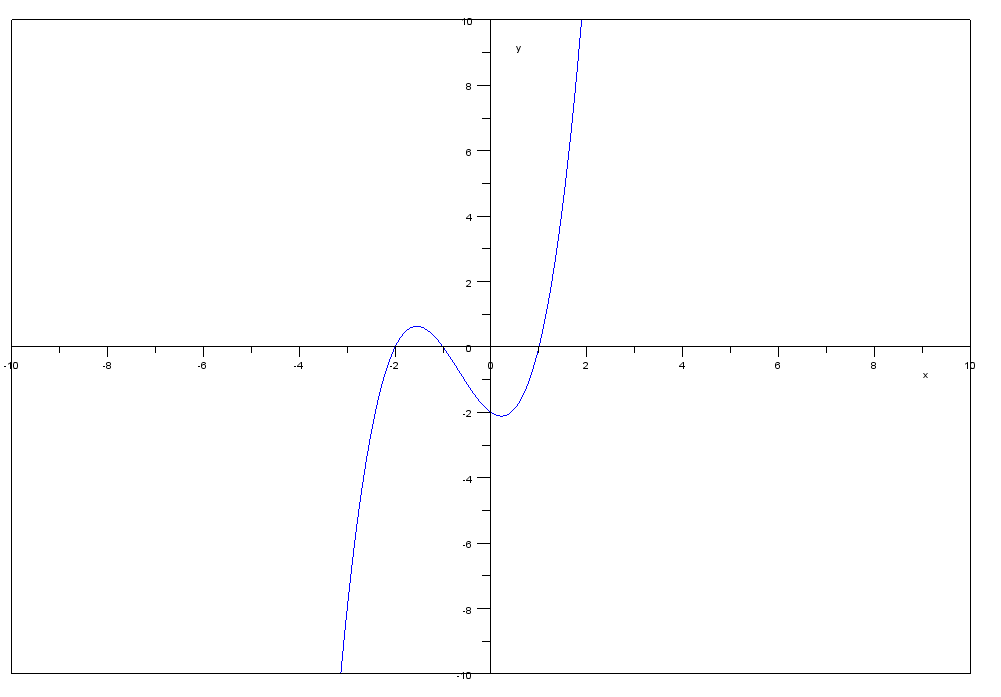
\includegraphics[width=0.8\textwidth]{03_pic04_1}
    \end{center}

\end{frame}
%-------------------------------------9. dia------------------------
\section{Integrálszámítás}
\subsection{Határozatlan integrál}
\begin{frame}[fragile]
    \frametitle{Határozatlan integrál}
    \begin{center}
        Adja meg az $f(x)=\displaystyle\frac{3}{x\ln^2(x)}$ függvény összes primitív függvényét!
    \end{center}
    \textbf{Megoldás}
    \begin{align*}
        \int\frac{3}{x\ln^2(x)}\mathrm{d}x & = \int\frac{3}{x}\ln^{-2}(x)\ \mathrm{d}x= \\
                                           & -3\ln^{-1}(x)=\frac{-3}{\ln(x)}+C          \\
    \end{align*}
\end{frame}
%-------------------------------------10. dia------------------------
\subsection{Területszámítás}
\begin{frame}[fragile]
    \frametitle{Területszámítás}
    Számolja ki az alábbi görbék által közrezárt korlátos síkidom területét!
    \begin{gather*}
        y=x^2-2x+2 \\
        \\
        y=14-x^2
    \end{gather*}
\end{frame}
%-------------------------------------11. dia------------------------

\begin{frame}[fragile]
    \frametitle{Területszámítás}
    \begin{itemize}
        \item Metszéspontok megkeresése:
              \begin{gather*}
                  \\
                  x^2-2x+2=14-x^2\\
                  2(x^2-x-6)=0\\
                  \Downarrow\\
                  x_1=-3;x_2=2
              \end{gather*}
        \item Metszéspontok megkeresése:
              \[
                  \displaystyle\int_{-3}^{2}
                  -2(x^2-x-6)\ \mathrm{d}x=\left[-\frac{2}{3}x^3+x^2+12x\right]^2_{-3}=\frac{95}{3}
              \]
    \end{itemize}
\end{frame}

\end{document}
